\section{进程运行状态转变过程}\label{ux8fdbux7a0bux8fd0ux884cux72b6ux6001ux8f6cux53d8ux8fc7ux7a0b}

分析完从进程/线程从创建到退出的整个过程,我们需要在从全局的角度来看看进程/线程在做整个运行过程中的运行状态转变过程。在执行状态转变过程中,ucore在调度过程总,并没有区分线程和进程,所以进程和线程的执行状态转变是一致的,分析的结果适合用户线程和用户进程的执行过程。

首先为了描述进程/线程的整个状态集合,ucore在kern/process/proc.h中定义了进程/线程的运行状态:

\begin{lstlisting}
// process's state in his life cycle
enum proc_state {
    PROC_UNINIT = 0,  // uninitialized
    PROC_SLEEPING,    // sleeping
    PROC_RUNNABLE,    // runnable(maybe running)
    PROC_ZOMBIE,      // almost dead, and wait parent proc to reclaim his resource
};
\end{lstlisting}

这与操作系统原理讲解的五进程执行状态相比,少了一个PROC\_RUNNING态(表示正在占用CPU执行),这是由于在ucore中,用current(基于proc\_strcut数据结构)进程控制块指针指向了当前正在运行的进程/线程PROC\_RUNNING态,所以就没必要再增加一个PROC\_RUNNING态了。那么那些事件或内核函数会触发状态的转变呢?通过分析uore源码,我们可以得到如下表示:

\begin{figure}[htbp]
\centering
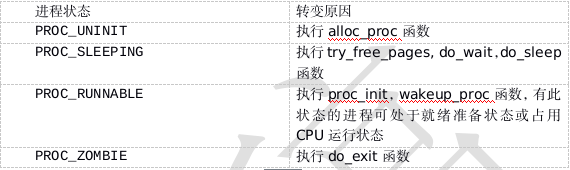
\includegraphics{figures/0_4.png}
\caption{0\_5}
\end{figure}

当父进程得到子进程的通知,回收完子进程控制块所占内存后,这个进程就彻底消失了。我们也可以用一个类似有限状态自动机来表示状态的变化:\lstinline!(需要用visio重画)!

\begin{lstlisting}
process state changing:

  alloc_proc                                 RUNNING
      +                                   +--<----<--+
      +                                   + proc_run +
      V                                   +-->---->--+ 
PROC_UNINIT -- proc_init/wakeup_proc --> PROC_RUNNABLE -- try_free_pages/do_wait/do_sleep --> PROC_SLEEPING --
                                           A      +                                                           +
                                           |      +--- do_exit --> PROC_ZOMBIE                                +
                                           +                                                                  + 
                                           -----------------------wakeup_proc----------------------------------
\end{lstlisting}

